\documentclass[pdftex,twocolumn,10pt,letterpaper]{extarticle}

%%% Set these variables appropriately
%%%
%% Note:  Authors is hardcoded below, this line only used for the PDF info
\newcommand{\AUTHORS}{Sol Boucher, Anuj Kalia, David G. Andersen, and Michael Kaminsky}
\newcommand{\TITLE}{Putting the "micro" back in microservice}
\newcommand{\KEYWORDS}{TODO}
\newcommand{\CONFERENCE}{USENIX ATC '18}
\newcommand{\PAGENUMBERS}{yes}       % "yes" or "no"
\newcommand{\COLOR}{yes}
\newcommand{\showComments}{yes}
\newcommand{\comment}[1]{}
\newcommand{\onlyAbstract}{no}

%%%%%%%%%%%%%%%%%%%%%%%%%%%%%%%%%%%%%%%%%%%%%%%%%%%%%%%%%%%%%%%%%%%%%


%%%
%%%  Fonts
%%%
\usepackage[T1]{fontenc}
\usepackage[utf8]{inputenc}
%\usepackage{textcomp}
\usepackage{newtxtext,newtxmath}       % Times/Times-like math symbols
\usepackage{bm}                        % bold math; use \bm{} in captions
\usepackage[scaled=0.92]{helvet}
\usepackage{courier}
%\usepackage[scaled=0.83]{beramono}    % more compact, good for code
%\usepackage{inconsolata}              % another nice alternative to courier


%%%
%%%  Page Setup
%%%
\special{papersize=8.5in,11in}
\setlength{\pdfpagewidth}{8.5in}
\setlength{\pdfpageheight}{11in}

\usepackage{ifthen}
\ifthenelse{\equal{\PAGENUMBERS}{yes}}{%
\usepackage[nohead,
            left=1in,right=1in,top=1in,
            footskip=0.5in,bottom=1in,     % Room for page numbers
            columnsep=0.25in
            ]{geometry}
}{%
\usepackage[noheadfoot,left=1in,right=1in,top=1in,
            footskip=0.5in,bottom=1in,
            columnsep=0.25in
	    ]{geometry}
}

%%%
%%%  Captions
%%%
\usepackage[font=bf]{caption}
%%  Space between figure and caption (assuming caption
%%  is below figure)
%\usepackage[font=bf,aboveskip=0pt]{caption} % SPACE
%%  Space between caption and body text of document
%\addtolength{\textfloatsep}{-7pt} % SPACE

%%%
%%%  Section headings
%%%
\usepackage{titlesec}
%\titlespacing{\paragraph}{0pt}{*1}{*1}      % SPACE
%\usepackage[compact]{titlesec}              % SPACE

%\titleformat{\section}%                     % ACM: caps + period (for 10pt doc)
%  {\bf\large\uppercase}{\thesection.\quad}{0pt}{}

%%% The following should mimic the 9pt ACM sig-alt style headings
%%%
%\titleformat{name=\section}%                 % ACM: caps + period (for 9pt doc)
%  {\bf\LARGE\uppercase}{\thesection.\quad}{0pt}{}
%\titleformat{name=\section,numberless}%      % ACM: for categores, etc.
%  {\bf\LARGE}{}{0pt}{}[\vspace*{-2pt}]
%\titleformat{\subsection}%                   % ACM
%  {\bf\LARGE}{\thesubsection\quad}{0pt}{}
%\titleformat{\subsubsection}%                % ACM
%  {\it\Large}{\thesubsubsection\quad}{0pt}{}

%%%
%%%  Lists
%%%
\usepackage{enumitem}
\setlist{itemsep=0pt,parsep=0pt}             % more compact lists

%%%
%%%  Header / Footer
%%%
\usepackage{fancyhdr}
\renewcommand{\headrulewidth}{0pt}

\ifthenelse{\equal{\PAGENUMBERS}{yes}}{%
  \pagestyle{plain}
}{%
  \pagestyle{empty}
}

%%%
%%%  Bibliography
%%%
\usepackage[numbers]{natbib}

%%%
%%%  Footnotes / Endnotes
%%%
\interfootnotelinepenalty=10000  % Split footnotes are annoying

% If you want endnodes, uncomment:
%\usepackage{endnotes}
%\usepackage{drafthead}
%\let\footnote=\endnote

%%%
%%%  Tables
%%%
\usepackage{booktabs}
\usepackage{color}
\usepackage{colortbl}
\usepackage{float}                           % Must appear before hyperref to
                                             % avoid weird PDF compile issues

%%%
%%%  PDF setup
%%%
\ifthenelse{\equal{\COLOR}{yes}}{%
  \usepackage[colorlinks,citecolor=blue]{hyperref}%         % for online version
}{%
  \usepackage[pdfborder={0 0 0}]{hyperref}%  % for paper (B&W) version
}
\usepackage{url}

\hypersetup{%
pdfauthor = {\AUTHORS},
pdftitle = {\TITLE},
pdfsubject = {\CONFERENCE},
pdfkeywords = {\KEYWORDS},
bookmarksopen = {true}
}

% Anonymize figure inclusion
% Requires pdfTeX version 1.40.17
\pdftrailerid{} %Remove ID
\pdfsuppressptexinfo15 %Suppress PTEX.Fullbanner and info of imported PDFs

% Uncomment next line if your printer outputs black
% boxes instead of drop shadows; older PDF interpreters
% in printers can't handle those PDF 1.5 features
%\pdfminorversion=3
%\pdfobjcompresslevel=2


%%
%% Figure placeholder macros
%%

\definecolor{placeholderbg}{rgb}{0.85,0.85,0.85}
\newcommand{\placeholder}[1]{%
\fcolorbox{black}{placeholderbg}{\parbox[top][1.5in][c]{0.95\columnwidth}{#1}}}


%%%
%%%  Misc
%%%
\usepackage[pdftex]{graphicx}
\usepackage{soul}
% this allows \st and friends to work with citations
\soulregister\cite7
\soulregister\ref7
\soulregister\pageref7

%\setlength{\parindent}{0pt}
%\setlength{\parskip}{\baselineskip}

%\clubpenalty=10000  % Don't allow orphans
%\widowpenalty=10000 % Don't allow widows

%%%
%%%  To appear/appeared in text on title page
%%%
\usepackage[absolute]{textpos}
\newcommand{\ToAppear}{%
\begin{textblock*}{\textwidth}(0.95in,0.4in)
\begin{flushright}
    %\noindent{\fbox{\textsf{Under submission---please do not redistribute.}}}
    %  --OR--
    \noindent{\small To appear in \textit{Proceedings of the XYZ}\\
    \noindent{\small \textit{Conference (XYZ'08)}, City, State, Month 2008}}
    %  --OR--
    %\noindent{\small In \textit{Proceedings of the XYZ}\\
    %\noindent{\small \textit{Conference (XYZ'08)}, City, State, Month 2008}}
\end{flushright}
\end{textblock*}
}

%%%
%%%  Sample ACM Copyright Block
%%%
\newfloat{acmcr}{b}{acmcr}
\newcommand{\AcmCopyright}{%
\begin{acmcr}
\parbox[b]{20pc}{%
\footnotesize
Permission to make digital or hard copies of all or part of this work
for personal or classroom use is granted without fee provided that
copies are not made or distributed for profit or commercial advantage
and that copies bear this notice and the full citation on the first
page.  To copy otherwise, to republish, to post on servers or to
redistribute to lists, requires prior specific permission and/or a fee.

{\em Conference}, Month Date--Date, Year, Location\\
Copyright 200X ACM X-XXXXX-XX-X/XX/XX ...\$5.00}
\end{acmcr}}

%%%
%%%  Comments
%%%
\newcommand{\note}[2]{
    \ifthenelse{\equal{\showComments}{yes}}{\textcolor{#1}{#2}}{}
}

% Change these to your own initials as you like...
\newcommand{\dga}[1]{\note{blue}{DGA: #1}}
\newcommand{\mk}[1]{\note{red}{MK: #1}}
\newcommand{\solb}[1]{\note{green}{SOLB: #1}}

\date{}
\title{\textbf{Putting the "micro" back in microservice}}
\author{{\large Sol Boucher*, Anuj Kalia*, David G. Andersen*, and Michael Kaminsky$^\dagger$}\\
{\em * Carnegie Mellon University \; $^\dagger$ Intel Labs}}

% This needs to be the last thing before \begin{document}
%\usepackage{microtype}  % SPACE

%%%%%%%%%%%%%%%%%%%%  START DOCUMENT  %%%%%%%%%%%%%%%%%%%%%%%%
\begin{document}

\maketitle

\ifthenelse{\equal{\PAGENUMBERS}{yes}}{%
  \thispagestyle{fancy}
}{%
  \thispagestyle{empty}
}

%\AcmCopyright
%\ToAppear

We introduce novel programming abstractions for isolation of both time and memory.
They operate at finer granularity than traditional primitives, supporting preemption
at sub-millisecond timescales and tasks defined at the level of a function call.
This resolution enables new functionality for application programmers, including
users of unmanaged systems programming languages, all without requiring changes to
the existing systems stack.  Despite being concurrency abstractions, they employ
synchronous invocation to allow application programmers to make their own scheduling
decisions.  However, we found that they compose naturally with existing concurrency
abstractions centered around asynchronous background work, such as threads and
futures.  We demonstrated how such composition can enable asynchronous cancellation
of
threads and the implementation of preemptive thread libraries in userland, both
regarded for decades as challenging problems.

\ifthenelse{\equal{\onlyAbstract}{no}}{%
\section{Introduction}
\label{sec:intro}

As the scope and scale of Internet services continues to grow, system designers
have sought platforms that simplify scaling and deployment.
Services that outgrew self-hosted servers moved to datacenter racks, then
eventually to virtualized cloud hosting environments.
However, this model only partially delivered two related benefits:
\begin{enumerate}
\item Pay for only what you use at very fine granularity
\item Scale up rapidly on demand
\end{enumerate}

\noindent
The VM approach suffered from relatively coarse granularity:  Its atomic compute unit
of machines were billed at a minimum of minutes to months.  Relatively long startup
times often required system designers to keep some spare capacity online to handle
load spikes.

These shortcomings led cloud providers to introduce a new model, known as
serverless computing, in which the customer provides \textit{only} their code,
without having to configure its environment.   Such ``function as a service''
(FaaS) platforms are now available as AWS Lambda~\cite{www-amazon-lambda}, Google
Cloud Functions~\cite{www-google-cf}, Azure Functions~\cite{www-microsoft-af}, and
Apache OpenWhisk~\cite{www-apache-openwhisk}.  These platforms provide a model in
which: (1)  user code is invoked whenever some event occurs (e.g., an HTTP
API request), runs to completion, and nominally stops running (and being
billed) after it completes; and (2)  there is no state preserved between
separate invocations of the user code.  Property (2) enables easy auto-scaling
of the function as load changes.

Because these services execute within a cloud provider's
infrastructure, they benefit from low-latency access to other cloud
services.  In fact, acting as an access-control proxy is a recurring microservice
pattern:\@ receive an API request from a user, validate it, then access
a backend storage service (e.g., S3) using the service's credentials.

In this paper, we explore a design intended to reduce the tension between two of
the desiderata for cloud functions:\@ low latency invocation and low cost.  Contemporary
invocation techniques exhibit high latency with a
large tail; this is
unsuitable for many modern distributed systems which involve
high-fanout communication, sometimes performing thousands of
lookups to handle each user request.  Because user-visible response time often
depends on the tail latency of the slowest chain of dependent
responses~\cite{Dean:cacm2013}, shrinking the tail is crucial~\cite{Jalaparti:sigcomm2013,
Xu:nsdi2013,Li:socc2014,Jeon:asplos2016}.

Thus we seek to reduce the invocation latency and improve predictability, a
goal supported by the impressively low network latencies available in modern
datacenters. For example, it now takes $<20\mu{}s$ to perform an RPC between two
machines in
Microsoft Azure's virtual machines~\cite{Firestone:nsdi2018}. We believe,
however, that fully leveraging this improving network performance will require
reducing microservices' invocation latencies to the point where the network is
once again the bottleneck.

We further hypothesize---admittedly without much proof for this chicken-and-egg
scenario---that substantially reducing both the latency and cost of running
intermittently-used services will enable new classes and scales of applications
for cloud functions, and in the remainder of this paper, present a design that
achieves this.  As Lampson noted, there is power in making systems 
``fast rather than general or powerful''~\cite{Lampson1983}, because fast
building blocks can be used more widely.

Of course, a microservice is only as fast as the slowest service it relies on;
however, recall that many such services are offered in the same clouds and
datacenters as serverless platforms. Decreasing network latencies will push
these services to respond faster as well, and new stable storage
technologies such as 3D XPoint (projected to offer sub-microsecond reads and
writes) will further accelerate this trend by offering lower-latency storage.

In this paper, we propose a restructuring of the serverless model centered around
low-latency: \textit{lightweight microservices} run in \textit{shared processes}
and are isolated primarily with language-based \textit{compile-time guarantees} and
\textit{fine-grained preemption}.

%% \subsection{Not yet rewritten}

%% At the time of writing, AWS Lambda, Azure Functions, and Google Cloud Functions
%% cap instance execution time to 5--10 minutes.

%% \solb{AK: I see you touched this recently.  Do you still want to see us say it (and
%% where)?  I currently mention penultimate section of Motivation and related work that
%% providers presently impose a limit, without actually saying what it is.}
%% \mk{This subsection seems out of place.}

\section{Providing Preemption}
\label{sec:preemption}

% \solb{I was thinking of basing the conclusion off this; maybe it should just
% \textit{be} there?}
% 
% \solb{Is it weird to have the following paragraph after we discuss isolation and
% preemption?  I can't think of where else it would go.}
% 
% Our system comprises (1) a central dispatch process that manages the compute node,
% receiving requests and assigning them to (2) a number of worker processes (one per
% dedicated compute core) via a shared memory region.  Each worker process runs a
% tight loop that polls on a ready bit in shared memory; once it finds work to be done,
% it sets itself up to catch any runtime panic and jumps into user code.  The worker
% process receives frequent \texttt{SIGALRM}s to ensure it never loses control of its
% CPU:\ in the associated handler, it checks how for long the current job has been
% running and ends any that has gone over budget.  The rest of this section covers the
% trust model and the preemption scheme.

% <snip>

%\paragraph{Preemption scheme}

The system must be able to detect and recover from microservices that, whether
maliciously or negligently, attempt to run for longer than permitted.  The two parts
of this problem are (1) regaining control of the CPU and (2) aborting and cleaning up
after the user code.

As proposed in Section~\ref{sec:motive}, regaining control of the CPU happens when a
signal (\texttt{SIGALRM}) from the kernel transfers control to the worker process's
handler.  The handler then checks how long the current microservice has been running
and decides whether it should be killed.  (We register the handler using the
\texttt{SA\_RESTART} flag to \texttt{sigaction()} so that any interrupted blocking
syscalls are restarted transparently.)  However, there remain three important
questions:

\paragraph{For how long should each microservice be allowed to run?}
%Consider a well-utilized but not overloaded compute node in which a user task
%is executing on each available core, but there is no backlog behind which an incoming task must wait.
Assume, as in Section~\ref{sec:motive}, that each core executes one user task at a
time and that all microservice
functions are pre-compiled and resident (warm invocation).
%The impact of microservice runtime on tail latency in 
%(This being preliminary work, any discussion of the cluster-level
%scheduling responsible for these theoretical conditions are outside the scope of
%this paper.)
%Furthermore, we'll assume an incoming microservice that is warm on each
%worker thread.
We define $L$ to be the desired invocation latency, $B$ to be the
runtime budget allotted to each microservice, and $r_c$ to be the remaining runtime
of the microservice on CPU $c$.  Thus, in the worst case (where all tasks are
executing for their entire allotted time) the probability that the incoming
microservice will have somewhere to run in time to meet the invocation
latency SLO is given by:
\begin{equation}
p(r_\textrm{min} \le L) = \sum\limits_{c \in C} p(r_c \le L) = \big| C \big| \frac{L}{B}
\end{equation}
Given the 14 cores in our setup and imagining we want to keep the 99\% tail,
$p(r_\textrm{min} \le L) = 0.99$, to an $L$ of 8~$\mu{}s$, we need to kill tasks
running for more than 113~$\mu{}s$.

\paragraph{How often should the handler execute (the \emph{quantum})?}
We showed at the end of Section~\ref{sec:motive} that microsecond-scale preemption is
\textit{achievable}, but can it be done \textit{efficiently}?  To find out, we wrote
a microservice that measures the throughput of computing SHA-512 hashes over 64 B of
data at a time.  We then subjected its worker process to \texttt{SIGALRM}s, varying
the quantum and observing the resulting hashing throughput.
Figure~\ref{fig:hashtput} illustrates that by a quantum of about 20 $\mu{}s$,
throughput had reached 90\% of baseline.  Considering this an acceptable performance
degradation, we adopt this quantum and prescribe a runtime budget of 93 $\mu{}s$ so
that we can always kill over-budget microservices in time to avoid violating our tail
latency SLO.

\begin{figure}
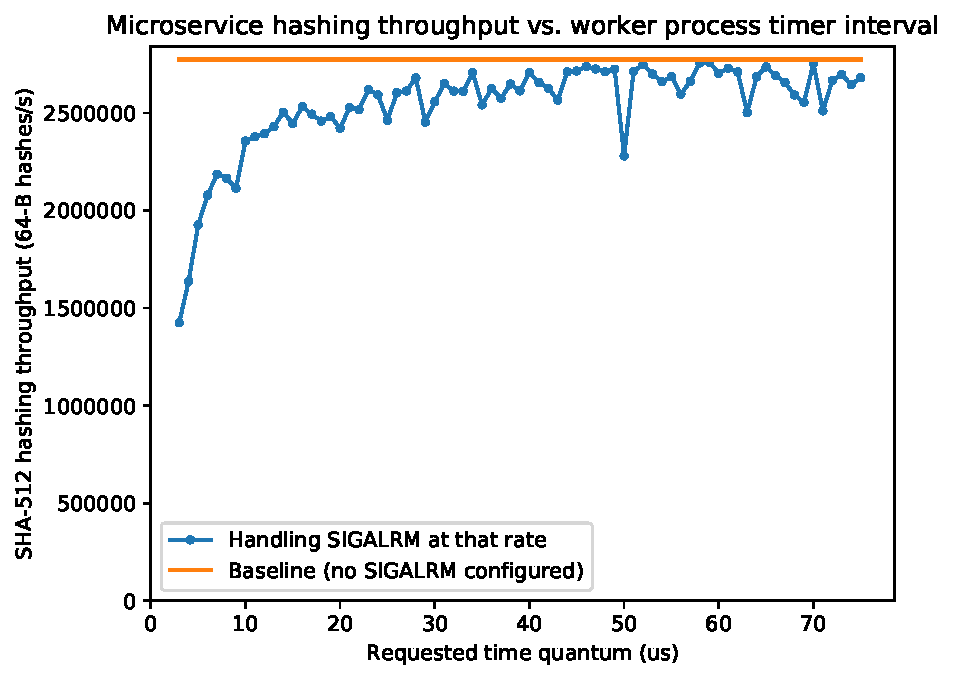
\includegraphics[width=\columnwidth]{figs/2018-02-02-evaluation_quantum-hasher_throughput-throughput}
\caption{Effect of \texttt{SIGALRM} quantum on SHA hashing throughput}
\label{fig:hashtput}
\end{figure}

\paragraph{How do we clean up a terminated microservice?}
We now discuss the mechanism for aborting
and cleanup.  POSIX signal handlers receive as an argument a pointer to their
\textit{context}, a snapshot of the process's PCB (process control block) at the
moment before it received the signal.  When the handler returns, the system will
transfer control back to the point described by the context, so a naïve way for our
worker processes to regain control would be to reset its GPRs (general-purpose
registers) to values recorded just before the worker's tight scheduling loop.
This approach, however, would not release the microservice's state or memory
allocations back to the worker.

One of the few heavyweight components of the Rust runtime is panic handling,
reminiscent of C++'s exception handling.  The compiler inserts landing pads into each
function that call the destructors for the variables in its stack frame, and if the
program ever panics,
the standard library unwinds the stack, jumping to each landing pad in turn.  We
co-opt this functionality by having the \texttt{SIGALRM} handler set its context
to describe executing a function that raises an explicit panic in a fake stack frame
just above the real top of the stack.

Section~\ref{sec:future} discusses several limitations and security
ramifications of this approach.

\section{Deployment}
\label{sec:deploy}

We now describe our microservices in the broader context of our full proposed
serverless system.  We clarify their lifecycle, interactions with the compute nodes,
and the trust model for the cloud provider.

Users submit their microservices in the form of Rust source code, allowing the
serverless operator to pass the \texttt{-Funsafe-code} compilation flag to reject
any \texttt{unsafe} code.  This process need not occur on the compute
nodes, provided the deployment server tasked with compilation runs the same version
of the Rust compiler\footnote{This restriction exists because, as of the latest
release (1.23.0) of the compiler, Rust does not have a stable ABI.}.  The operator
needs to trust the compiler, standard library, and any libraries against which it
will permit the microservice to link (since they might contain \texttt{unsafe} code),
but importantly need not worry about the microservice itself.

We believe that many users would find it acceptable to be presented with a specific
list of permitted dependencies.  But how big a list could the provider hope to offer
at the time of launching the service?  It bears noting that libraries including only
safe Rust code could be whitelisted without review.  To approximate how big such a
list would be given the current Rust ecosystem, we turn to a 2017
study~\cite{www-cratesio-unsafe} by the Tock authors that found just under half of
the Rust package manager's top 1000 most-downloaded libraries to be free of
\texttt{unsafe} code.  They caution that many of those packages have unsafe
dependencies, but we suspect that reviewing a relatively small number of popular
libraries would open up the majority of the most popular packages.

If the application compiles (is proven memory-safe) and links (depends only on
trusted libraries) successfully, the deployment server produces a shared object file,
which the provider then distributes to each compute node on which it might run.
Then, in order to ensure that invokers will experience the warm-start latencies
discussed in Section~\ref{sec:motive}, those nodes' host processes should instruct
one or more of their workers to preload the dynamic library.  If the provider
experiences too many active microservices for its available resources, it can
unload some libraries; on their next invocation, they will experience higher
(cold start) invocation latencies since we need to synchronously load the dynamic
library.  In our measurements, the overhead of this operation is about 100\textmu{}s.

\section{Related work}
\label{sec:related}

\begin{table*}
\small
\begin{tabular}{c||c|c|c|c|c|c}
&&& \multicolumn{2}{c|}{Dependencies} & \multicolumn{2}{c}{Third-party code support} \\
System & Preemptive & Synchronous & In userland & Works without GC & Preemptible & Works without recompiling \\
\hline
\textit{Scheme engines} & \checkmark* & \checkmark & \checkmark && $\dagger$ & --- \\
\textit{Lilt} && \checkmark & \checkmark && $\dagger$ & \\
\textit{goroutines} &&& \checkmark && $\dagger$* & --- \\
\textit{RT library} & \checkmark && \checkmark & \checkmark && --- \\
\textit{Shinjuku} & \checkmark &&& \checkmark & $\dagger$ & --- \\
\hline
\textit{libinger} & \checkmark & \checkmark & \checkmark & \checkmark & \checkmark & \checkmark
\end{tabular}

\centering{\checkmark* = the language specification leaves the interaction with blocking system calls unclear} \\
\centering{$\dagger$ = assuming the third-party library is written in a purely functional (stateless) fashion} \\
\centering{$\dagger$* = the third-party function must be written in Go and have no foreign depenedencies}
\caption{Systems providing timed code at sub-process granularity}
\label{tab:related}
\end{table*}

A number of past projects (Table~\ref{tab:related}) have sought to provide
bounded-time execution of chunks of code at sub-process granularity.
For the purpose of our discussion, we
refer to a portion of the program whose execution should be bounded as \textbf{timed
code} (a generalization of a preemptible function); exactly what form this takes
depends on the system's interface.

Interface notwithstanding, the systems' most distinguishing
characteristic is the mechanism by which they enforce execution bounds.  At one end
of the spectrum are \textbf{cooperative} multitasking systems where
timed code voluntarily cedes the CPU to another
task via a runtime check.  (This is often done implicitly; a simple example is a
compiler that injects a conditional branch
at the beginning of any function call from timed code.)
Occupying the other extreme are \textbf{preemptive} systems that externally
pause timed code and transfer control to a scheduler routine (e.g., via
an interrupt service routine or signal handler, possibly within the language's VM).

The cooperative approach tends to be unable to interrupt two classes of timed code:\@
(1) \textbf{blocking-call} code sections that cause
long-running kernel traps (e.g., by making I/O system calls),
thereby preventing the interruption logic from being run; and (2)
\textbf{excessively-tight loops} whose body does not contain any yield points (e.g.,
spin locks or long-running CPU instructions).
Although some cooperative systems refine their approach with mechanisms
to tolerate either blocking-call code sections~\cite{www-golang} or excessively-tight
loops~\cite{vanderwaart:cmucs2006}, we are not aware of any that are capable of
handling both
cases.

One early instance of timed code support was the \textit{engines} feature of
the Scheme 84 language~\cite{haynes:iucs1984}.  This added a new \texttt{engine}
keyword that behaved similarly to \texttt{lambda}, but created a special ``thunk''
accepting as an argument the number of ticks (abstract time units) it should run for.
The caller also supplied a callback function to receive the
timed code's return value upon successful completion.  Like the rest of the
Scheme language, engines were stateless:\@ whenever one ran out of computation time,
it would return a replacement engine recording the point of interruption.  Engines'
implementation relied heavily on Scheme's managed runtime, with ticks
corresponding to virtual machine instructions and cleanup handled by the garbage
collector.  Although the authors mention timer interrupts as an
alternative, this was apparently never tried.

\textit{Lilt}~\cite{vanderwaart:cmucs2006} introduced a language for writing
programs with statically-enforced timing policies.
Its compiler tracks the possible duration of each path through a program and
inserts yield operations wherever a timeout could possibly occur.  Although this
approach requires assigning the execution limit at compile time, the compiler is able
to handle excessively-tight loops by instrumenting backward jumps.
Blocking-call functions remained a challenge, however:\@ handling them would have
required
operating system support, reminiscent of \textit{Singularity}'s static language-based
isolation~\cite{hunt:msr2005}.

Some recent languages offer explicit userland threading, which could be used to
support timed
code.  One example is the Go language's~\cite{www-golang} \textit{goroutines}.
The language's runtime includes a cooperative scheduler that conditionally yields
at function call sites.  This causes problems with tight loops, the
traditional workaround being to manually add calls to the \texttt{runtime.Gosched()}
yield function~\cite{www-golang-tightloop}.

The solutions described thus far all assume languages with a heavyweight,
garbage-collected runtime.  However, some recent systems seek
to support timed code with fewer
dependencies.  One example is the userland C-language thread library for realtime
systems (here, ``\textit{RT}'') developed by Mollison and
Anderson~\cite{mollison:rtas2013}, which performs
preemption using timer interrupts, as proposed in the early Scheme engines
literature.  They install a periodic signal handler responsible for scheduling
tasks and migrating them between cores.  This lightweight runtime
achieves average overall scheduling latencies in the tens of microseconds;
however, as explained later in this section, the compromise is developer usability.

\textit{Shinjuku}~\cite{Kaffes:nsdi2019} is an operating system designed to perform
preemption at microsecond scale.  Built on the Dune framework~\cite{Belay:osdi2012},
it runs tasks on a worker thread pool controlled by a single centralized
dispatcher thread.  The latter polices how long each task has been running and
sends an inter-processor interrupt (IPI) to any worker whose task has timed out.
The authors study the cost of IPIs and the overheads
imposed by performing them within a VT-x virtual machine, as required by Dune.  They
then implement optimizations to reduce these overheads at the expense of Shinjuku's
isolation from the rest of the system.

As seen in Section~\ref{sec:intro}, nonreentrant interfaces are
incompatible with externally-imposed time limits.  Because such interfaces are
prolific in popular dependencies, no prior work allows timed code to transparently
call into third-party libraries.  Scheme engines and
Lilt avoid this issue by only supporting functional code, which cannot have shared
state.  Due to its focus on realtime embedded systems, RT assumes
that the timed code in its threads will avoid shared state; this mostly precludes
calls to third-party libraries, though the system supports the dynamic memory
allocator by treating it as specifically nonpreemptible.  Rather than dealing with
shared state itself, Shinjuku asks application authors to annotate any code with
potential concurrency concerns using a nonpreemptible \texttt{call\_safe()} wrapper.
And although Go is able to preempt goroutines written in the language
itself, a
goroutine that makes any foreign calls to other languages is treated as
nonpreemptible by the runtime's scheduler~\cite{www-golang-fficall}.

\section{Conclusion}

We presented the lightweight preemptible function, a composable new abstraction
for invoking a function with a timeout.  This enabled us to build a first-in-class
preemptive userland thread library by implementing preemption atop a cooperative
scheduler, rather than the other way around.  Our evaluation shows that lightweight
preemptible functions have overheads of a few percent (lower than similar OS
primitives), yet enable new functionality.

We believe the lightweight preemptible function abstraction naturally supports
common features of large-scale systems.  For example:  An ad renderer might implement
graceful degradation by rendering frames of an animation in a preemptible function,
dropping unfinished ones to meet its SLO.  An RPC server might preserve work by
processing each request in a preemptible function and memoizing the continuations; if
a request timed out but was later retried by the client, the server could resume
executing it from where it left off.


%\appendix
%\input{appendix_sources}

%\vspace{-0.1in}
%\section*{Acknowledgments}
% Comments for people we need to ack in the final version

%% Bibliography
\setlength{\bibsep}{2pt plus 1pt}  % plus 1pt seems to avoid widows/orphans
\small 
% \footnotesize % SPACE
\bibliography{biblio/ref}
\bibliographystyle{abbrvnat}
%\bibliographystyle{abbrvnat_noaddr} % SPACE
%\theendnotes % ENDNOTES
}{% !onlyAbstract
}

\end{document}

% Local Variables:
% TeX-command-default: "LaTeX PDF"
% End:

